\begin{equation}
    \begin{gathered}
        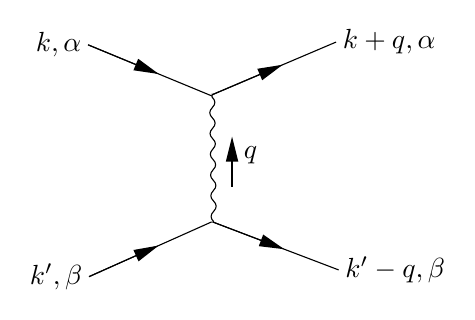
\begin{tikzpicture}[x=0.75pt,y=0.75pt,yscale=-1,xscale=1]
            %Straight Lines [id:da15915538235750892] 
            \draw    (100.17,172.51) -- (131.95,158.32) ;
            \draw [shift={(133.77,157.5)}, rotate = 515.9300000000001] [fill={rgb, 255:red, 0; green, 0; blue, 0 }  ][line width=0.08]  [draw opacity=0] (12,-3) -- (0,0) -- (12,3) -- cycle    ;
            %Straight Lines [id:da595892295722313] 
            \draw    (100.17,172.51) -- (159.26,146.12) ;
            
            %Straight Lines [id:da41375516068648066] 
            \draw    (160.29,146.04) .. controls (158.6,144.39) and (158.57,142.73) .. (160.22,141.04) .. controls (161.87,139.35) and (161.85,137.69) .. (160.16,136.04) .. controls (158.47,134.39) and (158.45,132.73) .. (160.1,131.04) .. controls (161.74,129.35) and (161.72,127.69) .. (160.03,126.04) .. controls (158.34,124.39) and (158.32,122.73) .. (159.97,121.04) .. controls (161.62,119.35) and (161.6,117.69) .. (159.91,116.04) .. controls (158.22,114.39) and (158.2,112.73) .. (159.84,111.04) .. controls (161.49,109.35) and (161.47,107.69) .. (159.78,106.04) .. controls (158.09,104.39) and (158.07,102.73) .. (159.72,101.04) .. controls (161.36,99.35) and (161.34,97.69) .. (159.65,96.04) .. controls (157.96,94.39) and (157.94,92.73) .. (159.59,91.04) .. controls (161.24,89.35) and (161.22,87.69) .. (159.53,86.04) -- (159.51,84.35) -- (159.51,84.35) ;
            %Straight Lines [id:da18427908684914152] 
            \draw    (159.7,146.12) -- (192.38,158.57) ;
            \draw [shift={(194.25,159.28)}, rotate = 200.85] [fill={rgb, 255:red, 0; green, 0; blue, 0 }  ][line width=0.08]  [draw opacity=0] (12,-3) -- (0,0) -- (12,3) -- cycle    ;
            %Straight Lines [id:da5517253733622631] 
            \draw    (159.7,146.12) -- (220.46,169.26) ;
            
            %Straight Lines [id:da9982758254698763] 
            \draw    (99.72,60.8) -- (131.97,74.12) ;
            \draw [shift={(133.82,74.88)}, rotate = 202.44] [fill={rgb, 255:red, 0; green, 0; blue, 0 }  ][line width=0.08]  [draw opacity=0] (12,-3) -- (0,0) -- (12,3) -- cycle    ;
            %Straight Lines [id:da26812450354509565] 
            \draw    (99.72,60.8) -- (159.69,85.57) ;
            
            %Straight Lines [id:da1756933542309722] 
            \draw    (159.57,84.84) -- (191.65,71.2) ;
            \draw [shift={(193.49,70.41)}, rotate = 516.96] [fill={rgb, 255:red, 0; green, 0; blue, 0 }  ][line width=0.08]  [draw opacity=0] (12,-3) -- (0,0) -- (12,3) -- cycle    ;
            %Straight Lines [id:da7638586957076614] 
            \draw    (159.57,84.84) -- (219.22,59.47) ;
            
            %Straight Lines [id:da9798265876333652] 
            \draw    (169.09,129.1) -- (169.09,107.04) ;
            \draw [shift={(169.09,105.04)}, rotate = 450] [fill={rgb, 255:red, 0; green, 0; blue, 0 }  ][line width=0.08]  [draw opacity=0] (12,-3) -- (0,0) -- (12,3) -- cycle    ;
            
            % Text Node
            \draw (97.72,60.8) node [anchor=east] [inner sep=0.75pt]    {$\boldsymbol{k} ,\alpha $};
            % Text Node
            \draw (221.22,59.47) node [anchor=west] [inner sep=0.75pt]    {$\boldsymbol{k} +\boldsymbol{q} ,\alpha $};
            % Text Node
            \draw (173.48,108.5) node [anchor=north west][inner sep=0.75pt]    {$\boldsymbol{q}$};
            % Text Node
            \draw (98.17,172.51) node [anchor=east] [inner sep=0.75pt]    {$\boldsymbol{k} ',\beta $};
            % Text Node
            \draw (222.46,169.26) node [anchor=west] [inner sep=0.75pt]    {$\boldsymbol{k} '-\boldsymbol{q} ,\beta $};
            \end{tikzpicture}
    \end{gathered} = - \frac{1}{\beta} \sum_{\omega_n} \int \frac{\dd[3]{\vb*{q}}}{(2\pi)^3} \frac{4\pi e^2}{\abs*{\vb*{q}}^2}.
\end{equation}